\documentclass[10pt,notes,compress,usetitleprogressbar,aspectratio=1610]{beamer}

\usepackage[english]{babel}
\usepackage[T1]{fontenc}
\usepackage[utf8x]{inputenc}
\usepackage[caption=false,font=footnotesize]{subfig} 		% Separar figuras en subfiguras

\usepackage{/home/vicdejuan/Imdea-S/tfg/definitions}

\newcommand{\pc}{\ensuremath{\mathit{pc}}\xspace}

\definecolor{palette1}{HTML}{1B9E77}
\definecolor{palette2}{HTML}{D95F02}
\definecolor{palette3}{HTML}{7570B3}
\definecolor{palette4}{HTML}{E7298A}
\definecolor{palette5}{HTML}{66A61E}
\definecolor{palette6}{HTML}{E6AB02}
\definecolor{palette7}{HTML}{A6761D}
\definecolor{palette8}{HTML}{666666}

\usetheme{metropolis}



\usepackage{tikz}
\usepackage{tikztools}
\usetikzlibrary{calc,shapes.multipart,chains,arrows,tikzmark,fit,shapes.geometric}



\title{First Order Proofs for Concurrent Programs}
\subtitle{Bachelor thesis | Double Degree Computer Science and Mathematics}
\author{Víctor de Juan Sanz}
\date{July 2016}
\institute{Imdea Software}

% \setbeameroption{hide notes}
% \setbeameroption{show notes}
% \setbeameroption{show only notes}


\newcommand{\PROGRAM}{\begin{array}{l@{\hspace{0.3em}}c@{\hspace{1em}}l}
		\hline
			l_1 & : & \mathtt{x := 10} \\
			l_2 & : & \mathtt{f := 1} \\
			l_3 & : & \mathtt{\textbf{while } (x\geq 1) \textbf{ do }} \\
			l_4 & : & \mathtt{\;\;f = f*x} \\
			l_5 & : & \mathtt{\;\;x=x-1} \\ 	
			l_6 & : & \mathtt{\textbf{end while}}\\
			l_7 & : & \mathtt{\cdots}\\
		\hline
		\end{array}}



\newcommand{\GOALS}{\varphi_1 \equiv \forall T(\pc(T) = l_5 \to \mathtt{x}\geq 1) \;\; \wedge \;\; \varphi_2 \equiv \mathtt{x} \geq 0}

\newcommand{\TRANSITIONS}{	\begin{array}{l}
		 \tau_1 \equiv\pc(T) = l_1 \andcond \pc\prime (T) = l_2 \andcond \mathtt{f\prime =f} \andcond \mathtt{x}\prime  = 10\\
		 \tau_2 \equiv\pc(T) = l_2 \andcond \pc\prime (T) = l_3 \andcond \mathtt{f}\prime  = 1 \andcond x\prime =x\\
		 \tau_3 \equiv\pc(T) = l_3 \andcond \pc\prime (T) = l_4 \andcond \mathtt{f\prime =f} \andcond x\prime \geq 1\\
		 \tau_4 \equiv\pc(T) = l_4 \andcond \pc\prime (T) = l_5 \andcond \mathtt{f}\prime  = \mathtt{f*x} \andcond \mathtt{x\prime =x}\\
		 \tau_5 \equiv\pc(T) = l_5 \andcond \pc\prime (T) = l_3 \andcond \mathtt{f\prime =f} \andcond \mathtt{x\prime =x-1}\\
		 \tau_6 \equiv\pc(T) = l_3 \andcond \pc\prime (T) = l_7 \andcond \mathtt{f\prime =f} \andcond \mathtt{x<1}
	\end{array}}


\begin{document}

\maketitle

\begin{frame}{Tabla de contenidos}
  \setbeamertemplate{section in toc}[sections numbered]
  \tableofcontents[hideallsubsections]
\end{frame}

%%%%%%%%%%%%%%%%%%%%%%%%%%%%%%%%%%%%%%%%%%%%%%%%%%%%%%%%%%%%%%%%%%%%%%
%%%%%%%%%%%%%%%%%%%%%%%%%%%%%%%%%%%%%%%%%%%%%%%%%%%%%%%%%%%%%%%%%%%%%%
%%%%%%%%%%%%%%%%%%%%		Motivation 			%%%%%%%%%%%%%%%%%%%%%%
%%%%%%%%%%%%%%%%%%%%%%%%%%%%%%%%%%%%%%%%%%%%%%%%%%%%%%%%%%%%%%%%%%%%%%
%%%%%%%%%%%%%%%%%%%%%%%%%%%%%%%%%%%%%%%%%%%%%%%%%%%%%%%%%%%%%%%%%%%%%%

\begin{frame}{Motivation}
	\begin{figure}
		\centering
		\includegraphics[scale=0.4]{imgs/japanesse.jpg}
		\caption{Japanese satellite lost in space: \$248 million.}
	\end{figure}
\end{frame}

\begin{frame}{Motivation}
	\begin{figure}
		\includegraphics[scale=0.9]{imgs/xray.jpg}
		\caption{XRay machine: Between 1985 and 1987 6 people died.}
	\end{figure}
\end{frame}

\begin{frame}{Motivation}
	\begin{figure}
		\centering
		\includegraphics[scale=0.8]{imgs/boeing.jpg}
		\caption{Boeing 787: \textit{failsafe} mode.}
	\end{figure}
\end{frame}



\begin{frame}{Objectives}
\begin{itemize}
	\item Prove correctness of an implementation of an ordered linked list.
	\begin{itemize}
		\item[--] Preservation as a list and order preservation.
	\end{itemize}
	\begin{figure}
		\newcommand{\Cross}{$\mathbin{\tikz [x=1.4ex,y=1.4ex,line width=.2ex, red] \draw (0,0) -- (1,1) (0,1) -- (1,0);}$}%

\newcommand{\Checkmark}{$\color{green}\checkmark$}


	\subfloat{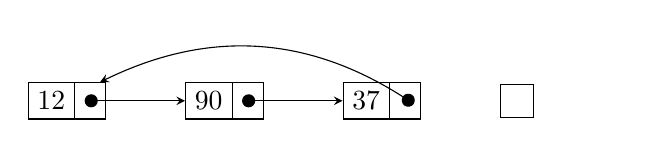
\begin{tikzpicture}[list/.style={rectangle split, rectangle split parts=2,draw, rectangle split horizontal}, >=stealth, start chain]
		  \node[list,on chain] (A) {12};
		  \node[list,on chain] (B) {90};
		  \node[list,on chain] (C) {37};
		  \node[on chain,draw,inner sep=6pt] (D) {$\fNull$};
		  \node at (7,0) (T) {\LARGE\Cross};
		  \draw[*->] let \p1 = (A.two), \p2 = (A.center) in (\x1,\y2) to (B);
		  \draw[*->] let \p1 = (B.two), \p2 = (B.center) in (\x1,\y2) to (C);
		  \draw[*->] let \p1 = (C.two), \p2 = (C.center) in (\x1 + 5.1,\y2-1.1) to[bend right] (A);
	\end{tikzpicture}}
	
	\vspace{0.4cm}

		\subfloat{
\begin{tikzpicture}[list/.style={rectangle split, rectangle split parts=2,draw, rectangle split horizontal}, >=stealth, start chain]
		  \node[list,on chain] (A) {12};
		  \node[list,on chain] (B) {90};
		  \node[list,on chain] (C) {37};
		  \node[on chain,draw,inner sep=6pt] (D) {$\fNull$};
		  \node at (7,0) (T) {\LARGE\Cross};
		  \draw[*->] let \p1 = (A.two), \p2 = (A.center) in (\x1,\y2) -- (B);
		  \draw[*->] let \p1 = (B.two), \p2 = (B.center) in (\x1,\y2) -- (C);
		  \draw[*->] let \p1 = (C.two), \p2 = (C.center) in (\x1,\y2) -- (D);
	\end{tikzpicture}}
	
	\vspace{0.4cm}

		\subfloat{
\begin{tikzpicture}[list/.style={rectangle split, rectangle split parts=2,draw, rectangle split horizontal}, >=stealth, start chain]
		  \node[list,on chain] (A) {12};
		  \node[list,on chain] (B) {37};
		  \node[list,on chain] (C) {90};
		  \node at (7,0) (T) {\LARGE\Cross};
		  \draw[*->] let \p1 = (A.two), \p2 = (A.center) in (\x1,\y2) -- (B);
		  \draw[*->] let \p1 = (B.two), \p2 = (B.center) in (\x1,\y2) -- (C);
	\end{tikzpicture}}
	
	\vspace{0.4cm}

	\subfloat{
\begin{tikzpicture}[list/.style={rectangle split, rectangle split parts=2,draw, rectangle split horizontal}, >=stealth, start chain]
		  \node[list,on chain] (A) {12};
		  \node[list,on chain,bend right] (B) {37};
		  \node[list,on chain] (C) {90};
		  \node[on chain,draw,inner sep=6pt] (D) {$\fNull$};
		  \node at (7,0) (T) {\LARGE\Checkmark};
		  \draw[*->] let \p1 = (A.two), \p2 = (A.center) in (\x1,\y2) -- (B);
		  \draw[*->] let \p1 = (B.two), \p2 = (B.center) in (\x1,\y2) -- (C);
		  \draw[*->] let \p1 = (C.two), \p2 = (C.center) in (\x1,\y2) -- (D);
	\end{tikzpicture}}
	\end{figure}
	\item[]
	\item[]
\end{itemize}
\end{frame}

\begin{frame}{Objectives}
\begin{itemize}
	\item Prove correctness of an implementation of an ordered linked list.
	\begin{itemize}
		\item[--] Preservation as a list and order preservation.
	\end{itemize}
	\begin{figure}
		\newcommand{\Cross}{$\mathbin{\tikz [x=1.4ex,y=1.4ex,line width=.2ex, red] \draw (0,0) -- (1,1) (0,1) -- (1,0);}$}%

\newcommand{\Checkmark}{$\color{green}\checkmark$}


	\subfloat{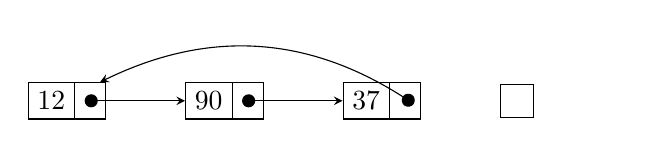
\begin{tikzpicture}[list/.style={rectangle split, rectangle split parts=2,draw, rectangle split horizontal}, >=stealth, start chain]
		  \node[list,on chain] (A) {12};
		  \node[list,on chain] (B) {90};
		  \node[list,on chain] (C) {37};
		  \node[on chain,draw,inner sep=6pt] (D) {$\fNull$};
		  \node at (7,0) (T) {\LARGE\Cross};
		  \draw[*->] let \p1 = (A.two), \p2 = (A.center) in (\x1,\y2) to (B);
		  \draw[*->] let \p1 = (B.two), \p2 = (B.center) in (\x1,\y2) to (C);
		  \draw[*->] let \p1 = (C.two), \p2 = (C.center) in (\x1 + 5.1,\y2-1.1) to[bend right] (A);
	\end{tikzpicture}}
	
	\vspace{0.4cm}

		\subfloat{
\begin{tikzpicture}[list/.style={rectangle split, rectangle split parts=2,draw, rectangle split horizontal}, >=stealth, start chain]
		  \node[list,on chain] (A) {12};
		  \node[list,on chain] (B) {90};
		  \node[list,on chain] (C) {37};
		  \node[on chain,draw,inner sep=6pt] (D) {$\fNull$};
		  \node at (7,0) (T) {\LARGE\Cross};
		  \draw[*->] let \p1 = (A.two), \p2 = (A.center) in (\x1,\y2) -- (B);
		  \draw[*->] let \p1 = (B.two), \p2 = (B.center) in (\x1,\y2) -- (C);
		  \draw[*->] let \p1 = (C.two), \p2 = (C.center) in (\x1,\y2) -- (D);
	\end{tikzpicture}}
	
	\vspace{0.4cm}

		\subfloat{
\begin{tikzpicture}[list/.style={rectangle split, rectangle split parts=2,draw, rectangle split horizontal}, >=stealth, start chain]
		  \node[list,on chain] (A) {12};
		  \node[list,on chain] (B) {37};
		  \node[list,on chain] (C) {90};
		  \node at (7,0) (T) {\LARGE\Cross};
		  \draw[*->] let \p1 = (A.two), \p2 = (A.center) in (\x1,\y2) -- (B);
		  \draw[*->] let \p1 = (B.two), \p2 = (B.center) in (\x1,\y2) -- (C);
	\end{tikzpicture}}
	
	\vspace{0.4cm}

	\subfloat{
\begin{tikzpicture}[list/.style={rectangle split, rectangle split parts=2,draw, rectangle split horizontal}, >=stealth, start chain]
		  \node[list,on chain] (A) {12};
		  \node[list,on chain,bend right] (B) {37};
		  \node[list,on chain] (C) {90};
		  \node[on chain,draw,inner sep=6pt] (D) {$\fNull$};
		  \node at (7,0) (T) {\LARGE\Checkmark};
		  \draw[*->] let \p1 = (A.two), \p2 = (A.center) in (\x1,\y2) -- (B);
		  \draw[*->] let \p1 = (B.two), \p2 = (B.center) in (\x1,\y2) -- (C);
		  \draw[*->] let \p1 = (C.two), \p2 = (C.center) in (\x1,\y2) -- (D);
	\end{tikzpicture}}
	\end{figure}
	\item  Formal verification of the correctness.
	\item Concurrent linked list (fine grain lock couple)
\end{itemize}
\end{frame}


\begin{frame}{Preliminaries}
\begin{itemize}
	\item We assume the usual way of representing and working with First Order Logic (FOL)
	\item Formal verification is proving correctness.... \textcolor{red}{LoL}
	\item We approach to assess correctness is by proving properties:
	\begin{itemize}
		\item Lifeness properties.
		\item \tikzmark{start1}Safety properties.\tikzmark{end1}
		\item Functional properties.
	\end{itemize}
	\begin{tikzpicture}[remember picture,overlay]
		\node<2,3>[draw,line width=2pt,orange,ellipse,inner ysep=8pt,fit={(pic cs:start1) (pic cs:end1)}] {};
		\node<3>[draw] at (5,1) {$\mathtt{x}≠0$};
	\end{tikzpicture} 
\end{itemize}
\end{frame}

\begin{frame}{Simple Programming Language (SPL)}
\note{\begin{itemize}
	\item Pre-estado y postestado.
\end{itemize}}
\[
	\begin{array}[t]{ll}
		\hline
		\text{Statement} & \text{Transition relation} \\ \hline\hline
		\begin{array}[t]{l@{\hspace{0.3em}}c@{\hspace{1em}}l}
			\ell_1 & : & \mathtt{\textbf{while } c \textbf{ do }} \\
			\ell_2 & : & \mathtt{\cdots} \\
			\mathtt{\vdots} \\
			\ell_n & : & \mathtt{\textbf{end while}} \\
			\ell_{n+1} & : & \mathtt{\cdots}
		\end{array}
		&
		\begin{array}[t]{ll}
				(\pc(T) = \ell_1 \andcond \;\;\texttt{c} \andcond \pc'(T) = \ell_2) \; 
				\orcond \\
				(\pc(T) = \ell_1 \andcond \lnot \texttt{c} \andcond \pc'(T) = 
			\ell_{n+1})
			& \text{for line $\ell_1$} \\ \\
			\pc(T) = \ell_n \andcond \pc'(T) = \ell_1 &
				\text{for line $\ell_n$}
		 \end{array} \\ \hline
	 \end{array}
\]
\end{frame}

\begin{frame}{Inductive Assertion Method}
\note{\begin{itemize}
	\item Un programa no concurrente, por ser un ejemplo más ilutrativo. 
	\item El objetivo es probar que hay fórmulas \textbf{invariantes}. 
	\item Es fácil ver que esto es cierto, tal y como lo tenemos aquí. Ilustramos el método con un ejemplo simple para que se entienda bien.
\end{itemize}}

	\begin{block}<1->{}
		\begin{center}
			\vspace{-1cm}
			\[
				\PROGRAM
			\]
		\end{center}
	\end{block}

	\begin{block}<2>{}
		\begin{center}
			
			\[
				\GOALS
			\]
		\end{center}
	\end{block}

	\begin{block}<3->{}
		\begin{center}
		\vspace{-4cm}
			\[
				\TRANSITIONS
			\]
		\end{center}
	\end{block}
\end{frame}


\begin{frame}{Inductive Assertion Method}
\note{\begin{itemize}
	\item En naranja, las condiciones de verificación.
	\item Si todas las condiciones de verificación son válidas, el candidato a invariante es un invariante.
\end{itemize}}
	\[
		\left.
			\begin{array}{ll}
				\textbf{Program:} 		&	 \PROGRAM \\\\
				\textbf{Transitions:}	&	 \TRANSITIONS \\\\
				\textbf{Goal : }	 	&	 \GOALS
			\end{array}
		\right\}
		\tikzmark{start2}
		\begin{array}{l}
			\tau_1 \andcond \varphi_i \to \varphi_i\prime  \\
			\tau_2 \andcond \varphi_i \to \varphi_i\prime \\
			\tau_3 \andcond \varphi_i \to \varphi_i\prime  \\
			\tau_4 \andcond \varphi_i \to \varphi_i\prime \\
			\tau_5 \andcond \varphi_i \to \varphi_i\prime  \\
			\tau_6 \andcond \varphi_i \to \varphi_i\prime 
		\end{array}
		\tikzmark{end2}
	\]
	\begin{tikzpicture}[remember picture,overlay]
		\node<2>[draw,line width=2pt,orange,square,inner ysep=64pt,fit={(pic cs:start2) (pic cs:end2)}] {};
	\end{tikzpicture} 

\end{frame}


\begin{frame}{Inductive Assertion Method}
	\paragraph{Some proofs for the invariance of $\varphi_1$:}
	\note{
	\begin{itemize}
		\item 1: Una cualquiera.
		\item 2: Claro, la interesante será en la que se modifica el valor de la x.
		\item 3: No, la interesante es la que llega a esa línea.
	\end{itemize}
	}

	\only<1>{\begin{block}{}
		 $\tau_2 \andcond \varphi_1 \to \varphi_1\prime $:
	%	\begin{dmath*}[indentstep={0em}]
		\begin{equation*}
			(
				\underbrace{\textcolor{black}{\pc(T) = l_2} \andcond \textcolor{orange}{\pc\prime (T) = l_3} \andcond \mathtt{f}\prime  = 1 \andcond x\prime =x}_{\tau_2} \andcond (\underbrace{\textcolor{black}{\pc(T) = l_5} \to \mathtt{x}\geq 1}_{\varphi_1})
			) 
				\to(\underbrace{\textcolor{orange}{\pc\prime (T) = l_5} \to \mathtt{x}\prime  \geq 1}_{\varphi_1\prime })\\\\
		\end{equation*}
	\end{block}}

	\only<2>{
	\begin{block}{}
	 	$\tau_5 \andcond \varphi_1 \to \varphi_1\prime $:
	%	\begin{dmath*}[indentstep={0em}]
		\begin{equation*}
		\begin{array}{r}
			(
				\underbrace{\pc(T) = l_5 \andcond \textcolor{orange}{\pc\prime (T) = l_3} \andcond \mathtt{f\prime =f} \andcond \mathtt{x\prime =x-1}}_{\tau_5} \andcond (\underbrace{\pc(T) = l_5 \to \mathtt{x}\geq 1}_{\varphi_1})
			) \\
				\to(\underbrace{\textcolor{orange}{\pc\prime (T) = l_5} \to \mathtt{x}\prime  \geq 1}_{\varphi_1\prime })\;\;\;\;
			\end{array}
		\end{equation*}
	\end{block}}

	\only<3>{\begin{block}{}
		 \;$\tau_4 \andcond \varphi_1 \to \varphi_1\prime $: 
		\begin{equation*}
			(
				\underbrace{\pc(T) = l_4 \andcond \pc\prime (T) = l_5 \andcond \mathtt{f}\prime  = \mathtt{f*x} \andcond \mathtt{x\prime =x}}_{\tau_4} \andcond (\underbrace{\pc(T) = l_5 \to \mathtt{x}\geq 1}_{\varphi_1})
			) 
				\to(\underbrace{\pc\prime (T) = l_5 \to \mathtt{x}\prime  \geq 1}_{\varphi_1\prime })\\\\
		\end{equation*}
		Equivalent to:
		\begin{equation*}
			(
				\mathtt{x\prime =x} \andcond  \mathtt{x}\geq 1
			) 
			\to (\mathtt{x}\prime \geq 1)
		\end{equation*}
	\end{block}}



\end{frame}

\begin{frame}{Inductive Assertion Method}
	\paragraph{Conclusion:}
		\begin{itemize}
			\item $\varphi_1$ is an \textbf{inductive invariant}.
		\end{itemize}
\end{frame}

\begin{frame}{Inductive Assertion Method}
	\paragraph{One proof for the invariance of $\varphi_2$:}

	\; $\tau_5 \andcond \varphi_2 \to \varphi_2\prime $:	
%	\begin{dmath*}[indentstep={0em}]
	\begin{equation*}
		(
			\underbrace{\pc(T) = l_5 \andcond \pc\prime (T) = l_3 \andcond \mathtt{f\prime =f} \andcond \mathtt{x\prime =x-1}}_{\tau_5} \andcond \underbrace{\mathtt{x} \geq 0}_{\varphi_2}
		) 
			\to \underbrace{\mathtt{x}\prime  \geq 0}_{\varphi_2\prime }\\\\
	\end{equation*}

	\only<2>{\begin{block}{}
		\begin{center}\textcolor{red}{\textbf{Counter example:}} $x=0$\end{center}
	\end{block}}
	\only<3>{\begin{block}{}
		\begin{center}$\varphi_1 \equiv \pc(T) = l_5 \to x ≥ 1$. Can we use that information?\end{center}
	\end{block}}
\end{frame}

\begin{frame}{Inductive Assertion Method}
	\textbf{Support:}


	\[
		(\textcolor{orange}{\tau_5 \andcond} \varphi_1 \andcond \varphi_2 \to \varphi_2\prime ) \rightarrow (\varphi_2\to\varphi_2\prime )
	\]

	\begin{block}<2->{}
	\vspace{-1cm}
		\textbf{We prove:}
		\begin{equation*}
			(
				\underbrace{\pc(T) = l_5 \andcond \pc\prime (T) = l_3 \andcond \mathtt{f\prime =f} \andcond \mathtt{x\prime =x-1}}_{\tau_5} \andcond \underbrace{\mathtt{x} \geq 0}_{\varphi_2} \andcond \underbrace{\pc(T) = l_5 \to \mathtt{x} \geq 1}_{\varphi_1}
			) 
				\to \underbrace{\mathtt{x}\prime  \geq 0}_{\varphi_2\prime }\\\\
		\end{equation*}
	\end{block}

	\only<3>{\begin{block}{}
		\vspace{-1cm}
		\textbf{Equivalent to:}
		\[
			( \mathtt{x\prime =x-1} \andcond \mathtt{x\prime }\geq 1) \to \mathtt{x} \geq 0 
		\]
	\end{block}}

	\only<4>{\begin{block}{}
		\vspace{-1cm}
		\textbf{Equivalent to:}
		\[
			( \mathtt{x\prime =x-1} \andcond \mathtt{x\prime }\geq 1) \to \mathtt{x} \geq 0 \;\;\LARGE\textcolor{green}{\checkmark}
		\]
	\end{block}}

\end{frame}

\begin{frame}{Problem}
\includegraphics[scale=0.15]{../graphics/listcode}
\end{frame}

\begin{frame}{Axioms}
\end{frame}



\begin{frame}{Times}
\end{frame}


\begin{frame}{Conclusions}
\end{frame}




\end{document}
